\chapter{Tin Can}
\label{ch:tincan}

In the introduction, I argued that taking a ``beyond being there'' approach to designing collaborative interactions can yield powerful results. I have shown in the past two chapters how designs that aim not to create the experience of ``being there'' but instead to imagine new kinds of relationships and interactions can be both meaningful to users and improve on traditional ``being there'' approaches to mediated interaction. In this chapter, I will introduce \emph{Tin Can}, a tablet-based application to collaborativly track discussion topics and ideas in a seminar-style discussion classroom. Based on our study of this system, I will argue that we have created a system that remains quite useful even when everyone using the system is face-to-face and could eschew the system entirely if it wasn't useful to them. Looking forward,  \citet{Hollan:1992tz} argue in 1992 that ``no one seems to be asking the question, ``what would happen if we were to develop communication tools with a higher information richness than face-to-face?'''' I view \emph{Tin Can} as one of many potential answers to this question.

In a classroom using \emph{Tin Can}, each student uses his or her own tablet to share text ideas in a synchronized, visual environment. The system is designed to promote diverse participation and increase engagement. Using this platform, we observed twelve class sessions and conducted interviews with the participating students. Instead of simply introducing an additional text-based communication channel into the classroom, we find that the system creates a new ``stage'' (in the Goffman sense) on which students could perform in ways that the main spoken stage could not support. This stage coexists with spoken communication, and augments how students attend to the material and each other. We conclude that spoken participation alone poses barriers for some participants and the addition of a non-oral, text-based stage can help establish more equitable, diverse, and engaging discussions in the class.

% the other options for this are "Computer-supported cooperative work" or "Collaborative computing". Bit of a wash which one we do.

\section{Introduction}

The physically co-located small group discussion is often viewed as the gold standard for effective collaboration and communication.  It can provide a space for participants to voice their opinions and can readily lead to deliberation and collective problem solving \citep{Burkhalter:2002vg}. Not surprisingly, it is often the case that designers seek to virtually reproduce the characteristics and norms of the small group discussion in technologically mediated communication media. \citet{Hollan:1992tz} provide a valuable counterpoint to this approach arguing against viewing experiences mediated by the ``physically proximate'' reality as necessarily superior to those mediated by technology. We have adopted the following challenge: instead of assuming that the small group discussion is good enough and the only appropriate design consideration is its preservation and replication, we seek to appropriately apply the unique properties of a technological system to the established affordances of a small group discussion. We would not deny that face-to-face interaction offers many substantial benefits when compared to interactions mediated by, for instance, a video conferencing system; nevertheless, we argue that there is room to improve the physically proximate small group discussion by intervening in the assumed normal frameworks of turn-taking and attention. \sidenote{Much of the contents of this chapter are drawn from \citep{Harry:2012df}, which represents collaboration between the author of this dissertation and Eric Gordon.}

In this paper, we describe the design and enacted use of a tablet-based system for a discussion-based graduate seminar. Although this is not a common educational venue for intervention (lecture classes are a more traditional venue, e.g. \citep{Kam:2005wb} or \citep{Bergstrom:wl}), it is one in which we identified a number of potential problems with pure face-to-face discussions that a tablet-based system might effectively address. We had two major goals for this work: first, create a class discussion context that encouraged more diverse participation in class; and second, to help students feel engaged and connected to the learning environment. 

To meet these goals, we sought to expand notions of legitimate participation beyond speaking, using the affordances of a text-based communication system. Our system creates an alternate communication space within the learning environment. Typically, in group communication contexts, spoken participation is viewed as the primary or dominant interaction medium, one that is often the target of modification as in, for example, \emph{Second Messenger}\citep{DiMicco:2007ie} or \emph{Meeting Mediator}\citep{Kim:2008ip}. Like the \emph{Cognoter}\citep{Tatar:1991jq} system, our system placed emphasis on the combinatory possibilities of text-based and oral participation in a co-located group communication environment.  Unlike \emph{Cognoter}, however, we focus on enhancing the performative space of group interaction. Consequently, our goal was not to create alternative communication channels; instead, it was to expand the space of performance. As part of this conceptual shift, we argue for moving from the metaphor of a ``front'', spoken channel and a ``back'' channel to the metaphor of a ``main'' performance stage and ``side'' performance stage.

This study seeks to understand how having simultaneously accessible stages in the context of a group discussion affects the methods and outcomes of participant engagement. We start by describing how our system, called \emph{Tin Can}, is related to existing systems that similarly augment face-to-face communication. We introduce the idea of \emph{stages} and contrast it to previous models of \emph{channels}. We then describe in detail the critical design elements of the \emph{Tin Can} application and the class context in which it was implemented. Then, we present the results of the study, based on class observations, process traces, and interviews.  In our discussion, we return to the concept of stages and describe how this formulation of participation can be productive for thinking through how people can interact with additional stages introduced into the dominant context of face-to-face communication. Finally, we discuss some specific insights about the tablet as a platform and describe the extent to which the design met our initial goals and how our results compare to those from past findings in the literature.


\section{Related Work}


% REVISION Unnecessary, I think.
% We situate our work amongst three related categories of systems: systems that augment face-to-face discussions, systems designed for classroom engagement, and systems to support backchannel conversations. We will relate this work to ours both in terms of design as well as (when appropriate) experimental findings.

% we'll include nunamaker etc in that category
% From Chapanis: "A final point of interest is that a subject is much more likely to take control of a voice channel than of a channel or any combination of channels lacking voice." (41-42).  

There is a rich field of research on the topic of augmenting co-present group communication with socio-technical systems.  One significant area of investigation concerns how systems can ``level the playing field'' of face-to-face communication through reflecting information about a group's behavior back on itself. \citet{Karahalios:hu} refer to this as a ``social mirror''; a real-time visualization of social dynamics that is shared by the whole group and can cause changes in group dynamics. They suggest that ``social mirrors become another channel for interaction (or a back channel) and, in the process, become a signal that influences interaction.'' Their exemplar social mirrors measure behavior in an audio channel and visualize different aspects of it on on shared Displays.\sidenote{There are a series of projects in this stream, including table-top interfaces for visualizing machine-recognized topics \citep{Bergstrom:2009fe}, reaching consensus through discreet voting \citep{Bergstrom:2009ej}, or balancing relative participation in group conversations \citep{Bergstrom:2007je}.} This strategy is shared by \emph{Second Messenger}\citep{DiMicco:2007ie} and \emph{Meeting Mediator}\citep{Kim:2008ip}.  In these systems, presenting real-time participation visualizations tended to close the gap between over-participating group members and under-participating members, although in most cases this effect was primarily from over-participating members decreasing their participation. This work demonstrates how visualizing main stage spoken participation in different ways can impact relative participation rates by encouraging individuals to censor or otherwise alter the nature of their communication to correspond with perceived group norms and group behavior.

Another strain of this work is less interested in altering the oral channel of group communication, and more focused on creating separate, productive  backchannels. There are a variety of contexts where people have added communication channels. \citet{Yardi:2006uk} describes how a chat-based backchannel operates over a semester in a class, \citet{mccarthy_digital_2004} describe a similar approach at a conference. This early work focuses on characterizing the kinds of use that occur in backchannels using existing systems like chat, but do not engage specifically with design issues in backchannels. \citet{Harry:2009jh} propose a new design for projecting question-oriented backchannels in panel presentations.  \citet{Yankelovich:2005bx} discuss oral backchannels during remote, audio-conference-based meetings, and the ``social translucence'' research stream (\emph{Rendezvous} \citep{kellogg_leveraging_2006} is most closely related to this work) explores the design of systems to represent engagement in different kinds of mediated social situations.

\emph{Tin Can} is designed specifically for use in a class, and is thus influenced by the systems designed for this specific context. Like much of the backchannel work described above these systems are typically concerned with creating new channels for communication in, for example, a large lecture hall. Bergstrom's lecture class system \citep{Bergstrom:wl} supports question-asking and commenting and the \emph{Livenotes} project \citep{Kam:2005wb} supports taking shared notes on lecture presentation slides. The \emph{ActiveClass} project \citep{Ratto:2003vs} creates a channel between students and instructors for asking anonymous questions during a lecture from PDAs.  Each of these systems seeks to increase participation in very large group settings by establishing separate channels for participation.  Work in this space is typically not focused on directly influencing spoken participation because the expectation is that there is none; the lecturer is (except for question-asking) the only legitimate participant.

% not going to mention Classroom2k because it's about archiving and we're not talking about that now.
\emph{Classroom 2000} \citep{Abowd:1998wp} created a ubiquitous computing environment to create rich records of a lecture. \emph{Tin Can} shares \emph{Classroom 2000}'s interest in generating a record of the class, but takes a decidedly low-sophistication approach to it, relying on members of the class to generate the appropriate metadata instead of a broad technical infrastructure. Although questions play a role in our system as well, they are in-the-moment guides to discussion and not primarily aimed at the professor (indeed, the professor asked many of the questions in the system). \emph{Classroom 2000} is focused primarily on lecture situations, which have very different interaction dynamics than the discussions \emph{Tin Can} supports. \emph{Classroom 2000} focused on adding value (in our terminology) to the main stage performances of the professor, and are not trying to create credible side stages for student interaction.

In \emph{Tin Can}, we take a different approach. We seek to expand the stage of participation by diversifying the sites of performance. In other words, we are not interested in creating better oral or better text-based channels; instead, through their correspondence, we seek to create a rich environment for participation composed of multiple, simultaneous stages.   Perhaps the earliest research to explore this sort of approach is \citeapos{Tatar:1991jq} work on \emph{Cognoter}. They pointed to some interesting problems with creating stages, namely the limits of the ``parcel-post'' model of communication---where a message is sent and subsequently received and interpreted. Although this model works well for written correspondence, they found that within \emph{Cognoter}, because the written contributions were designed to be interspersed with verbal dialogue, it was difficult for users to understand them ``within the time frame of the actual communication'' unless the oral conversation paused while written contributions were processed. In other words, in actual practice, users resorted to channel switching in order to accommodate the written or the oral modes. Another example is the \emph{Thoughtswap} \citep{DickeyKurdziolek:2010wt} project which takes a much more structured approach by interspersing periods of engagement with the system with freeform discussion. In \emph{Tin Can}, we employed a similar model of written communication to \emph{Cognoter} and \emph{Thoughtswap}, but we found that we were able to successfully create simultaneous stages for participation instead of stages one at a time. We will discuss the reasons for this disparity at more length in the conclusions. Work in this space on how alternate communication channels are selected and used owes a clear debt to \citeapos{Ochsman:1974vu} early work on mediated collaboration.

%These systems are focused on adding back or side stages to existing main stages. In contrast, Nunamaker's work on brainstorming and decision-making \cite{nunamaker_electronic_1991} seeks to create a new main stage for the group that strongly structures verbal interaction.



% The early work in this area was most concerned with supporting existing tools or methods for achieving backchannels in various social situations, particularly presentations,  lectures, and meetings. Yardi describes how a chat-based backchannel operates over a semester in a classroom \cite{Yardi:2006uk}, McCarthy et al. describe a similar approach at a conference \cite{mccarthy_digital_2004}. This early work focuses on characterizing the kinds of use that occur in backchannels using existing systems like chat, but do not engage specifically with design issues in backchannels.  

% We are in many ways inspired by the work of DiMicco et al. on \emph{Second Messenger} \cite{DiMicco:2007ie}. The notion of

% I want to work this in somewhere, but since the shift away from focusing on systems it makes less sense here. 
% \emph{Tin Can} also supports significantly more participants than any of these systems, which has major impacts on the kinds of dynamics at work.

% This is a design-oriented way of contrasting the work. Going to try to spend less time on that in this rewrite.
% \emph{Tin Can} shares some of these visualization strategies and is supported by their findings that discussants can feasibly attend to and respond to representations of their interactions while maintaining a conversation. It differs, though, in the level of activity it expects from its users. \emph{Tin Can} offers a distinct communication framework and active curation in contrast to the machine learning techniques frequently employed in these kinds of systems. \emph{Tin Can} also supports significantly more participants than any of these systems, which has major impacts on the kinds of dynamics at work.


% saving these references in case we need them, but we don't reallly need to go that cite-crazy here. better to spend or space on other stuff.
% as described by Karahalios \cite{Bergstrom:hu} 

% REVISION This should be slimmed down in a revision of the related work section, since we're taking the focus off creating an archive. Also, it should focus more on more closely related stuff like livenotes, Bergstrom's backchan.nl like system, and cognoter. 








% 

%  

% REVISION This is a bit wordy. I might try to trim this pretty substantially and just defer the whole conversation to when we actually dig in on the difference. In any event, I think this is either a decent way to introduce the discussion here, or we can salvage it when we do the full discussion later.






% All of these projects share \emph{Tin Can}'s interest in creating new spaces for group communication, and some of these kinds of systems are integrated into the physical spaces the group inhabits. Backchannels are not just focused on co-located groups, however, and Kellogg \cite{kellogg_leveraging_2006} (among others, like \cite{Yankelovich:2005bx}) has addressed how text and audio backchannels can operate in distributed contexts. Most of this work focuses on backchannels as a generalized communication channel, but some researchers, like Nunamaker, focus instead on building formalized systems for brainstorming and decision-making to which (like \emph{Tin Can}) each user has dedicated personal access, but (unlike \emph{Tin Can}) attempt to use the mediated backchannel to structure and drive the front channel interactions \cite{nunamaker_electronic_1991}.


\section {Setting the Stage}

The research questions and goals for the students' experience using \emph{Tin Can} are captured in the main stage / side stage model. We wanted to create a side stage experience where participation was viewed as a legitimate part of class discourse and had a clear impact on the oral discussion. This is in some ways a radical strategy: why should we add technology to a classroom discussion if we want people to be more involved and attentive?


% COMMENT The paragraph that follows is really great. I love that way of framing the problem. (Drew)

\begin{figure*}[t]
\centering
\includegraphics{figures/tincan/tincan_interface.png}
\caption{A screenshot of the \emph{Tin Can} interface running on a tablet.}
\label{f:interface}
\end{figure*}

Traditionally, educators have accepted the quality and sufficiency of the main stage in small groups and eschewed the addition of other communication channels because they might be distracting. A seminar class already adheres to the gold standard of face-to-face communication. It is often assumed that the pressures of the performance are exactly what we want them to be---students talk and the professor evaluates. But there are two faulty assumptions here.  The first is that engagement in a co-present discussion can be manifested only in established methods of performance, for example, speech. And the second is that all students are equally capable of convincing performances. Social psychology research suggests that introverts rely more heavily on written communication to express themselves \citep{Ross:2009gp, Wilson:2010ib}. But when there is only one legitimate kind of performance in a class, when there is only one way to perform on the front stage, the structure of the learning environment may not be as equitable as it could be, and it may not even be as productive as possible, even for extroverts. 

Consequently, when designing for the seminar, we sought to intervene in the established norms of the front stage by adding a well-crafted additional stage. The goal was to create a context for the legitimate performance of the back stage without having to \emph{go away} from the front stage.  As such, we move away from the front/back distinction, preferring the notion of a main stage with a side stage. We sought to design a system where performers could be on both stages at once, where performances were simultaneous, not alternating. Furthermore, the front and back stage as Goffman uses it implies different audiences for front and back performances. Moving to main and side stages reinforces the shared audience of the two stages, which has a big influence on how people perform on each stage and makes it easier to integrate those performances in a meaningful way. We use the terms main stage (face-to-face, spoken conversation) and side stage (text input) to explain the context of performance created as a result of using \emph{Tin Can}.  

% REVISION Try to bring in that quote from the cognoter paper? "Our construction of this distinction is that whiteboard items hold a dual status as elements in the conversation and elements that may be conversed about"
% This quote captures part of the distinction we're going for here. Whiteboards, like Tin Can, occupy a space where they have the same audience as the verbal conversation but are a distinct space with distinct affordances.

%In our research context, the seminar classroom, this conceptual structure is problematic because of the unique performative nature of the space. In a small group discussion, there is no front and back. The act of speaking, typically a required component of a seminar class, is both a method of personal engagement in a topic and a performance that can be evaluated by the professor and fellow students. Even when not speaking, there is a sense of being on stage, as students feel compelled to perform their attentiveness.  This is notably distinct from a large lecture classroom where, presumably, when not speaking, a student can retreat into the background or engage in an alternative channel. 

%It is our belief that many other small group situations beyond the classroom share this structure and when designing systems for these environments it is valuable to consider the stage model instead of a channel model. By recognizing the fluidity of potential performance options for everyone involved and the subtle ways people can select and use different stages for their messages, we open up a broader design space than a model of separate or irreconcilable channels would offer.

% REVISION Knocked this out for now, since Twitter is probably not the right way to lead into backchannels because it's a fringe use of Twitter and we don't want people to think TWITTER IS A BACKCHANNEL or something (like one of the reviewers did). 
% For example, Twitter has become a popular technology employed at academic conferences and in classrooms to enable participants to communicate outside of the dominant stream of communication, whether that be a lecture or panel presentation \cite{Gabriel:2011vz}.


%This metaphor of alternating stages has been influential to the thinking about alternating channels in large group situations, but it does not adequately extend to the social context of a small group.  While in traditional backchannel configurations each group (presenter/audience) has only one channel for communication at their disposal, everyone in a small group context is both a potential presenter \emph{and} audience member. This makes the channel model somewhat limiting because it is primarily oriented towards broadcasting and depends on the asymmetry of a front/back distinction that does not really exist in a small group context. 




% may not need the backchannl cite here - it's kind of an outlier. probably remove it and focus on stuff that's more core like yardi + boyd. 

% note to self - lots of other citations we can drop in here about backchannel conceptions, including a ref to the original meaning of backchannel that is lost with modern usage of the term. Drew has this stuff relatively close to the surface and will add it in later.

% Going to play down the nod line stuff a bit. My main concern here is that I don't want to use the nod line as a dividing line between situations where this kind of system would/wouldn't work, and I don't want to conflate it with small/large group size distinctions, either. So what's it useful for? 

% We understand the small group discussion as existing below what Erving Goffman calls the ``nod line.'' \cite{Goffman_Nod_Line} This is the imaginary line that separates small communities from large ones. In communities of a particular size, member are compelled to nod to everyone they pass.  Once a community gets too large, this is no longer practical or even desirable. In a below-the-nod-line community, members know each other by name and are compelled to communicate this fact when encountering others in the community.  Whereas in large, above-the-nod-line communities, the responsibility for interpersonal acknowledgement is lessened, and as such, the nature of communication is distinct.  We are specifically interested in how this is manifested in the large lecture classroom versus the small seminar classroom.  We argue that the metaphor of channels in below-the-nod-line situations is not appropriate, as the intimacy of these situations cannot accommodate wholly alternative communication streams.  Instead, below-the-nod line situations can accommodate a texturing of attention through what we call \emph{stages}.   

% there's a bit of a two-component argument going on here - backchannel as a term describes one particular configuration of a computer mediated communication environment, and we really want to limit it to that and not have it seep out into other potential configurations like this one where it's not as meaningful. 


% can we get some citations of this being a concern in education literature? 
% also, curious if we can find some citations of teacher-practice-oriented attempts to address the issue. harkness discussion structures come to mind, but I suspect there are others out there. 


% Note to self: say something about why perhaps why channels had been the historical metaphor of choice? My instinct is this has to do with the asymmetry of situations where backchannels are traditionally deployed: because it's the ONLY channel the audience can perform on, there's a tension between making a system that satisfies the audiences desire for a primary, full-featured medium (like chat) and something that serves as an effective meeting point between the audience and presenter (which is what backchan.nl aspires to be). As a result, our discourse tended to support the one-channel model over the multiple-stages model because those were the kinds of systems we were looking at.







\begin{figure*}[t]
\centering
\includegraphics{figures/tincan/classroom_overview.png}
\caption{The classroom environment. The student at the head of the table is presenting and controlling the projector. The professor is to the presenter's right.}
\label{f:classroom}
\end{figure*}

% Commented out, since we're not talking much about the archive to save space.
% \begin{figure}[t]
% \centering
% \includegraphics[width=3.25in]{figures/tincan/archive.png}
% \caption{A screenshot of the archive document generated at the end of the class.}
% \label{f:archive}
% \end{figure}

\section{System Design}
 
\emph{Tin Can} is a tablet-based application to support class discussions. It provides a synchronous environment shared by the students and professor and each user has his or her own tablet. Students are physically co-located with the professor. Students arranged their tablet in different ways. Some keep them on their laps, some on the table in front of them. All users (including the professor and researcher) have the same capabilities in the system. The system serves as a visualization of the current state of the group discussion. It focuses on three main parts of a class's process: topics, time, and ideas. Figure \ref{f:interface} shows the interface in action.\footnote{A video of the interface and the classroom context is available at \url{http://www.youtube.com/watch?v=ztVllLuCcTM}}

\subsection{Topics}
The topics pane in the UI collects past, current, and potential future discussion topics. These topics can be added using the ``Add Topic" button at the bottom of the pane. The current topic is highlighted in a topic-specific color. All topics have a short text description. Past and current topics show a kind of clock pie chart, illustrating the start and end times of a discussion topic (or the current time in the case of ongoing topics). The total duration in minutes of past and current topics is also shown as part of the topic text. Topics can be tapped to bring up an interface for changing their state: starting future topics, stopping current topics, and restarting past topics. 

\subsection{Time}
The clock in the center of the screen serves as a reminder both of the current time as well as a concise visual representation of the history of discussion topics covered in the class. The time spent on each topic is swept out radially on the clock such that large blocks of color represent topics that occupied a longer period of the class. When an hour of time has passed, the central area in the clock is cleared and the colored record of the previous hour appears at the edge of the clock. Up to four hours can be easily represented in this way. The clock is non-interactive. 


\subsection{Ideas}
The ideas pane contains a time-sorted list of ideas. An idea is simply a text contribution. Although we had presumptions about what would be posted here (as indicated by the terminology we used in the interface), ideas evolved to include statements, questions, recording main stage discussion themes, and a simple Twitter-like reply syntax. When entering an idea, the author of the idea could do one of two things: ``add idea" or ``add idea to group." The former option would store the idea in the user's ``personal" idea drawer.  The latter option would immediately put the idea at the top of the group idea timeline, as well as adding it to their personal drawer. Users tap and hold to ``like'' an idea. The idea flashes and a ``+$X$'' notation appears in its text, where $X$ is the number of likes that the idea has received in total. Ideas in the group timeline have their author's name displayed in parentheses after the text of the idea. Ideas are colored based to match the color of the current topic. 

\subsection{Users}
Each user logged in to the system is displayed on a tab around the edge of the screen. The arrangement is essentially random. Tapping a user extends that user's idea drawer. This drawer contains all ideas created by the user, whether shared or not. These ideas are differentiated in the list by ``(shared)" being appended to ideas that have been shared. Any unshared idea in the idea drawer can be dragged from the drawer to the group idea area, even if the user didn't originally author the idea. Ideas dragged by other people are attributed differently in the main timeline. For example, an idea created by Alice and shared by Bob would say ``(Alice, shared by Bob)". By design, personal folders are not private.  They are semi-public spaces meant to give users some choice in how their contributions are read by the group.

\begin{figure*}[p]
\centering
\includegraphics{figures/tincan/archive.png}
\caption{A screenshot of the post-class archive.}
\label{f:archive}
\end{figure*}


\subsection{Archive}
All ideas and topics are recorded on the server. At the end of each class session, the server emails everyone who attended the class with a list of their personal ideas and a link to a shared Web page that include a list of all student ideas sorted by topic and by user.

An example of such an archive is shown in figure \ref{f:archive}.




\section{Research Context and Methods}
We deployed the \emph{Tin Can} system in two sections of a graduate seminar on media and social theory taught by one of the authors \sidenote{Recall that the work of this chapter was a collaboration with Eric Gordon, as published in \citep{Harry:2012df}; he was the professor in this class.} at a liberal arts college. One section met in the morning, the other in the afternoon, twice a week. Class assignments were reading-based. Each discussion class was usually lead by a student or pair of students. While what it meant to lead class changed somewhat over the course of the study, the pre-study norm was to prepare a slideshow and accompanying media (images and video were quite common) and present it to the class. The morning session had eight regular students and the afternoon session had eleven regular students. In total, thirteen students were male, six were female. There were five non-native English speakers in both classes. 

Our study lasted for six weeks and utilized mixed methods, including classroom observations, capture of text inputs, and semi-structured interviews.

Throughout the deployment, user interactions were captured. This did not, notably, include live recording of class audio, only text-based interactions with the \emph{Tin Can} system itself. We made the decision not to record audio because we felt that this would make students self-conscious and would be too disruptive to main stage interactions.  In lieu of audio recordings, for most class sessions, a researcher other than the professor was present to observe the class. We employed a form of direct observation known as continuous monitoring, where the researcher documented everything he saw throughout the study period, including the description of the environment and participant actions, as well as inferences about their meaning \citep{interpersonal_interaction}. The researcher's observations were not prescribed before the study, because of the exploratory nature of this first deployment. We did not know what to expect, so the observations were designed to be generative and not conclusive.  We documented patterns of student attentiveness to peers and professor; interactions with tablets (i.e. position of tablets on the table or in laps); and correlations between speaking and writing. The students were aware that their use of \emph{Tin Can} was being studied and they were aware of the presence of the researcher. Because the students were invested in the use of \emph{Tin Can}, the presence of the researcher was not disruptive, but instead added to the excitement they had about testing a new system.  The field notes were recorded by hand and subsequently transcribed and shared with the teaching researcher. 

All text inputs into \emph{Tin Can} were recorded over 22 hours of usage across twelve class sessions.  Each class was about two hours long, but classes often had a non-discussion logistical content from the professor at the beginning of sessions. The average \emph{Tin Can} session was 105 minutes long. After the deployment, the inputs were categorized into types, including topics and ideas, shared and non-shared.

Finally, at the conclusion of the discussion-based component of the class, the researchers conducted semi-structured individual interviews with fifteen of the nineteen students ($79$\%). Interviews were conducted by the non-teaching researcher to alleviate student concerns about sharing judgements about the teaching researcher, although there were no sections of any of the interviews that students did not want to be shared with the teaching researcher. All interviews were recorded and transcribed and entered into \emph{Dedoose}, a qualitative analysis tool. Because we view this work as generative, we iteratively coded the transcribed interviews, letting themes (and codes) arise organically as we reviewed the interview data, observational data, and process traces from the class. This strategy closely resembles \citeapos{Glaser:1967tj} grounded theory approach. All names mentioned in interviews or shown in screenshots have been obscured or changed to pseudonyms to protect the identities of those participating in the research.

% REVISION Knocked this paragraph out for space. Was just connective tissue and I think we'll do okay without it. 
In the results section to follow we will analyze the kinds of content entered into \emph{Tin Can}.  The discussion section will then connect the interviews and observations to these findings.  


\section{Process Traces}

\begin{figure*}[p]
\centering
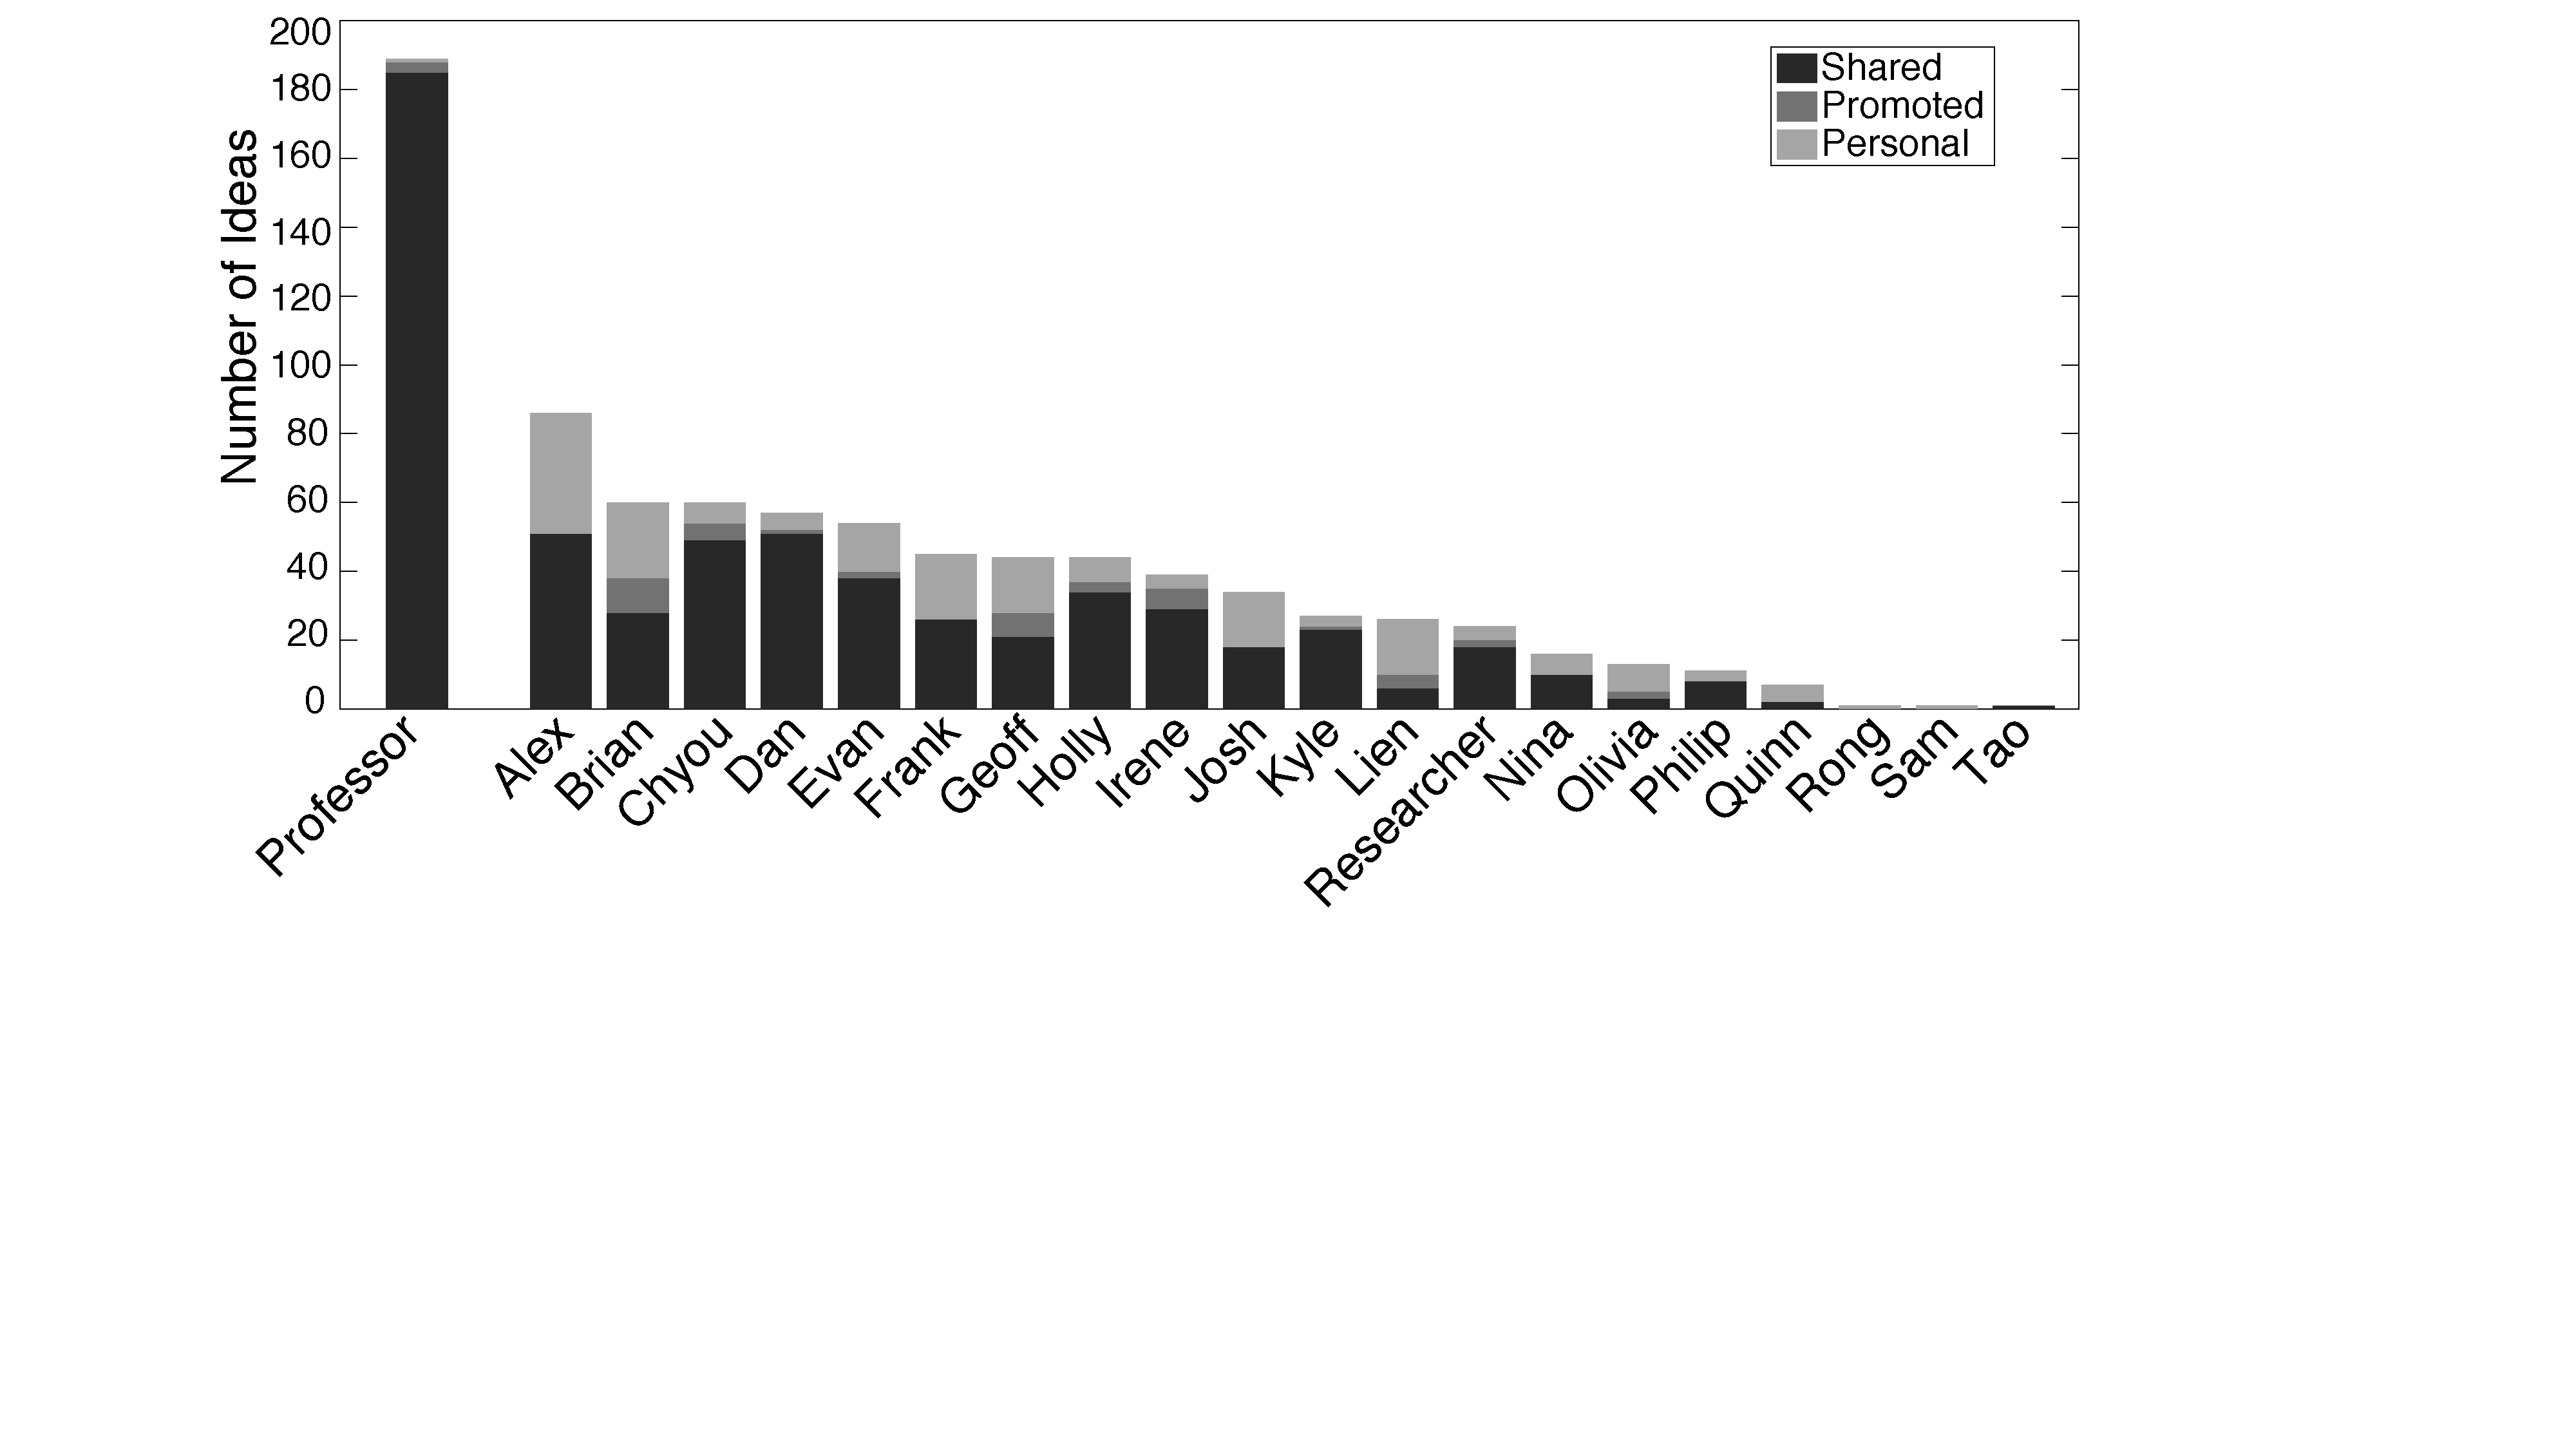
\includegraphics{figures/tincan/ideas_per_participant.pdf}
\caption{Distribution of ideas per participant per idea type: personal, promoted, and shared.}
\label{f:ideas_per_participant}
\end{figure*}

\begin{figure*}[p]
\centering
\includegraphics{figures/tincan/timeline.pdf}
\caption{Timeline of topics and ideas posted in two example class sessions. Ideas posted by students are in black, ideas from the professor are in red. The height of the line indicates the length (in characters) of the idea. Topic names are shown above their corresponding section of the class.}
\label{f:class_timelines}
\end{figure*}


Over the course of the deployment of \emph{Tin Can}, 839 ideas and 119 topics were created. The  majority of ideas created were shared: $72\%$ of ideas were shared on creation. Another $5\%$ were personal ideas that were turned into public ideas by being dragged by another user from a user's personal idea drawer to the public idea area. The balance, $23\%$ of ideas, were never shared. The distribution of these different idea types on a per participant basis can be found in figure \ref{f:ideas_per_participant}. 

Over the course of the study, 119 topics were created in total. Of these, 79 were actually discussed and the remainder were raised as potential topics but never actually used. The average class had 6.5 started topics, with a standard deviation of 2.3. Topic duration had a much wider variation: the average topic lasted 851 seconds with a deviation of 673 seconds. This is skewed largely because of very short topics. 

A deep analysis of temporal patterns within the data is beyond the scope of this paper, but to provide a rough sense of what topic and idea posting activity looked like we have provided two example timelines in figure \ref{f:class_timelines}. The most striking thing about the data from this perspective is that the temporal distribution is very uneven. In Kleinberg's terms, we see a bursty structure \citep{Kleinberg:2003ej} in idea posting. This is a common structure in communication systems and it is no surprise that it appeared in our study results. 

% REVISON I don't think we need this. In what follows, we present some summary statistics of topic and idea use during class, discuss some of its temporal properties, and describe a rough set of categories that capture the diversity and relative frequency of student ideas in \emph{Tin Can}.





%WHAT WOULD YOU SAY ABOUT CUTTING OUT THE ENTIRE IDEAS SECTION? I'M NOT SURE IT IS NEEDED.
%REVISON I don't think we need this sentence. We intentionally provided little guidance, beyond the name itself, for what the ideas section of the interface was intended. 


\subsection{Ideas}

Over the course of the semester, ideas were adapted for many different purposes. Based on a review of the captured ideas, we organized them into a set of broad categories.

Statements were the most common type of idea. Statements capture an argument or idea, like ``Talking about sex is a means of controlling it.'' These contributions are similar to what someone might say if they had a speaking turn. Alternatively, they sometimes represented note-taking behavior. Students were also particularly fond of ``X vs Y'' dualisms, which we describe as Theme ideas. Like statements, these often had a dual purpose of either proposing a useful dualism or capturing the nature of the current discussion. 

Questions were about half as common as statements. They usually took a rhetorical form, like ``Where do you draw the line between not being sexually repressive and being excessively open about it?'', or were framed as less forceful variants of statements like ``Is identity a sign? Or is it that which is signified?''

Early in the study, students developed techniques to address their ideas at specific other students. Using ``@'' syntax, as in ``@dan, I don't think the two are mutually exclusive.'' they could respond to other students' ideas non-orally.


\section{Discussion}
Much of the existing literature on backchannels focuses on situations in which the audience has one stage to perform on and the presenter has a separate one.  \citep{Yardi:2006uk, mccarthy_digital_2004} \emph{Tin Can}'s symmetry, where anyone can use either stage at any time, is the focus of our analysis. In this section, we use the stages metaphor introduced earlier to describe how students managed their attention to stages. Then, we discuss how students made decisions about when and how to perform on the available stages. 

\subsection{Attention}
% Attention, for our purposes, is best understood not as an innate characteristic of someone's behavior, but as a value-laden socially situated performative behavior. ``We are always to a certain extent in a state of distraction,'' according to sociologist Emile Durkheim. \citep{Durkheim:1974tc} Every situation is composed of stimuli that disrupts some fictional conception of undivided attention.  Likewise, every situation requires some aspect of performance, as individuals are required to communicate their attentiveness in response to specific social contexts.

As described in Chapter \ref{ch:background}, attention is best understood as a socially situated performative behavior. In a lecture, attentiveness is typically demonstrated by looking at the presenter and potentially taking notes. In a small group discussion, attentiveness might be expanded to include looking through class reading material or looking at other people. 


Traditional approaches to managing attention in education tend to take as their starting point the desire to maximize audience attention on the presenter through the physical architecture of lecture spaces, presentation media, and rhetorical strategies. \citet{Gordon:2009us} argue that attention and distraction are best understood as being ``hand-in-hand. The very same new technologies and landscapes that cultivate a state of distraction are themselves directed simultaneously toward the cultivation of attention.'' Educators tend to look to technology (broadly construed) to help manage overwhelming sensory inputs while simultaneously blaming the lack of attention of students on that same technology.

% cite giddens here? I do love the structure + enactment stuff, but I'm not sure it's something we can just drop in here unless it's other places too and gets a paragraph introducing it to people who might be unfamiliar with it. 

Of course, it is not simply a definitional matter to decide what constitutes attention in a class using \emph{Tin Can}. To understand how students and professor understood attention in this context we can look to how they talked about attention and distraction. Students predominantly viewed participation as obligatory. Speaking to his motivation to use \emph{Tin Can}, one student said ``to be part of the class I had to use it.'' Students were never admonished for interacting with tablets, and didn't report feeling like they needed to minimize their performance on the side stage to avoid negative perceptions of themselves by the professor or others, except to the extent that students felt like over-participation on either stage might crowd out other students. A student who was particularly active on the side stage worried that ``I take so much space that people that are shy...have more problems ... standing up when they have personal ideas [to share].''

%QUESTION: is that quote above accurate?  It doesn't make much sense?

To the extent that students were concerned with attention, the most common problem was not being viewed as inattentive, but struggling to track performances on both stages simultaneously. Although students were not concerned with annoying the professor, they were worried about offending their peers who were presenting that day: ``It is a little tough to keep your attention on both [stages], and sometimes you get a running conversation on \emph{Tin Can}, which can be interesting but it is maybe a little unfair to the presenter.'' Although this perspective represents a pull towards enacting traditional models of attention, it wasn't enough to significantly diminish involvement (either as a performer or an audience member) on the side stage. Student presenters often used \emph{Tin Can} as a way to gauge interest in future discussion topics and to decide on whom to call.

In resolving the conflict between compelling simultaneous performances, students could fall back on the persistence of performances on the side stage. In making a choice to attend to the main stage, they could, in Josh's words, ``have a comfort that you're not going to miss anything because you can always go back and see other people's posts whenever.'' Still, there seemed to be a difference between browsing posts later and being part of the live conversation. This came up most frequently when students expressed frustration with text entry on the tablet and missing the right moment to post something: ``I didn't get it out as fast as I'd hoped and it was already passed and it wasn't worth typing it anymore.'' 

%Although posts would be available for reading later, there was still a sense of timeliness and not attending to the side stage represented a sort of sacrifice of opportunities for performance. 

% TODO could chop that last clause, I guess.

Deciding between stages was really only a problem when both stages were compelling. If only the main stage was compelling, students could freely attend to that. The reverse was also common, and students frequently reported attending to the side stage as an escape from an un-engaging main stage, as in this quote from Quinn:
\begin{quote}
``I can remember a particular ... presentation that he was doing a lot of PowerPoint, I think he was completely oblivious to the \emph{Tin Can} conversation and [the \emph{Tin Can} conversation] ended up going in a very good direction ... as a result, I do not remember anything he said, because ... the conversation on \emph{Tin Can} was a little more engaging''
\end{quote}


% REVISION I want to make this point somewhere, but I'm not sure exactly where to do it. I sort of what it earlier, but if it's before the performative attention argument it might feel a little adrift. 

%This is great.  I like the paragraph here.

Moments like this highlight the extent to which our characterization of stages as ``main'' and ``side'' is itself a product of attention. The presence of a system like \emph{Tin Can} does not automatically create a side stage, nor does the ability for spoken communication guarantee that such communication will create a main stage.  The addition of a mediated communication platform simply creates the \emph{possibility} of a new stage. Whether or not it becomes a viable stage, and whether the mediated stage is a main stage or a side stage is all the result of people's attention to and actions in the system. Furthermore, the designation ``main'' or ``side'' is not fixed. The situation Quinn describes is a moment where the main stage ceased, for a little while, to command people's attention and \emph{Tin Can} took on some main stage properties. Although such moments were rare, they point out how stages are not created by technology or decree: they are designated and sustain by the collective attention and action of people using them.


The professor's high level of activity on \emph{Tin Can} throughout the class can be seen as playing a role in setting the main/side distinctions. His activity was a way of giving students permission to take the side stage seriously, both because it was clear that he was going to notice contributions from students, but also because he was frequently entering ideas himself and not looking at the current speaker. This underlines the extent to which this was an ideal context for testing a system like \emph{Tin Can}. Had we deployed in a class where the professor was neutral or hostile to people attending to \emph{Tin Can}, traditional class expectations of attention would more likely have been practiced by students, reinforcing those norms and making a side stage much less viable.




% I think I want a paragraph here about how the professor viewed attention, but not sure how to attack it. I want to say something about how the professor's high activity level + framing of participation on TC as "part" of the class as playing an instrumental role in expanding the boundaries of potential attentive behavior. I think we can see this in the "role of the professor" codes. People talk about viewing participation as "mandatory" or "expected", which I think suggests that they had explicit permission from you to see use of the system as part of positive participation. 

% not sure if we want to include this, but figured I'd spit out a first pass paragraph for it.

% This is a nice story, but I don't think we have room for it here. 
% -----------------------------
There was a moment towards the end of our study when the professor brought in a colleague over video chat to discuss his work and answer questions from the class. The remote presenter had a very limited view of the room from the professor's laptop video camera and could see only a few students. Although the \emph{Tin Can} system was available for this section of the class, it went almost entirely unused. This may simply be because the activity on the main stage was engrossing, but the total lack of side stage performance was still well outside of the bounds of normal disuse during a particularly engaging presentation in class. This suggests to us that the students were concerned with enacting the traditional model of attention for this outsider to the class. He could have viewed intense tablet use (something that was normal and viewed as attentive during normal class sessions) as inattentive or disrespectful and so his presence (even though his view of the classroom was quite limited) triggered a reversion to the more restrictive expectations of attention in a traditional class context.

% I like this too, but this doesn't add a whole lot and isn't that strong.
% -----------------------------
During class sessions, we also conducted focused observations of student attention. The researcher would pick a student and mark down when they changed what they were looking at. Although this was not comprehensive data for all students, when students weren't looking at the current speaker they were predominantly concerned with their own bodies and clothing, not the tablet. The tablet hardly dominated their attention. Even among the most active users of \emph{Tin Can}, their attention was usually on the speaker and shifted to the tablet during periods of silence or topics they found less interesting. When the professor spoke, students were far more likely to look at him than when other students were speaking. 

\subsection{Performance}

The presence of an additional participation stage complicates the experience of being a member of the class. When should you submit an idea on the tablet rather than say it out loud? When is the right time to say something? Should you share an idea or make it a personal idea? The enacted (and self-reported) answers to these questions can provide some insight into the experience of using the system as well as deepen our understanding of the stages metaphor. In many cases, students viewed the side stage as complementing the main stage and valued its presence in situations where a range of problems with the main stage impeded their participation. In this way, \emph{Tin Can} acted as a kind of escape valve: when the main stage was working for people, they used it; when they felt like they could not use it or did not want to use it, they turned to the side stage and valued its complementary affordances.

Performance on the main stage was widely viewed as more challenging and having higher stakes than side stage performance. Among the students who were reluctant oral participants in class, this was particularly acute. Geoff, a very rare oral participant in class before \emph{Tin Can}, was particularly frank on this point: ``I don't really talk a lot in class because I'm scared of sounding stupid.'' Geoff was a more frequent side stage participant. Although he would still rarely speak up directly in class, he was often called on by others in class to speak about ideas he had posted on \emph{Tin Can}; he would happily speak in those instances. This change in behavior on his part was frequently brought up by other students as being a major benefit of using \emph{Tin Can} because they valued the opportunity to hear and see what he was thinking. Irene, a more talkative student, characterized Geoff as a member of a ``good chunk of people who I think are thinkers and they would just think and write down what they were thinking'' as opposed to speaking on the main stage. This feeling was common among people who were comfortable on the main stage, who acknowledged that ``not everyone feels comfortable speaking in class, so I think [\emph{Tin Can}] definitely allowed for certain ideas to be shared that probably would have been either suppressed or just ignored or forgotten.''

Students' comfort with the different properties of the main stage and side stage influenced which stage they chose for a performance. Students for whom English was a native language were more comfortable in spoken conversation, and when faced with complex ideas preferred to express them orally, turning to \emph{Tin Can} to express simpler ideas because typing complex ideas was slow. Students who did not speak English natively had the reverse logic, preferring to type complicated ideas so they could, according to Rong, ``organize my language a lot before I actually talk because I want my thoughts to be systematical and clear, I want people to get it.'' In both groups, though, students viewed the revisability of written contributions as a potential benefit: ``[\emph{Tin Can}] gave me the advantage of thinking it through in a writing sense a little bit before I vocalized the idea.''

A lack of confidence about one's performances was not the only reason to choose the side stage over the main stage. Students had a clear sense of etiquette surrounding when they could participate on the main stage and in what ways. Because only one person could be talking at once and conversations were fundamentally linear, students often felt like speaking up themselves would be changing the flow of the conversation in an inappropriate way. Instead, students would prefer to write their comments on the side stage instead of ``interrupting'' on the main stage. This was intertwined with ideas of timeliness. Performances seen as being closely related to the current main stage conversation were more appropriate than performances that might drag the conversation in a significantly different direction. Although similar, these concerns are not precisely the same. The worry about interruption was primarily a desire to not unduly influence the path of the conversation because that was perceived by some students as the role of the professor or presenter, not the role of the individual student. In contrast, ideas that were seen as ``not quite as relevant [and not] really [fitting] into the conversation'' were not really valid performances on the main stage at all because not only would they move the conversation significantly, they did not necessarily have anything to do with the existing main stage conversation.

Both of these worries, though, led to the same thing: increased use of the side stage. Because turn-taking was not a concern on the side stage, it easily supported ideas going in different directions simultaneously. To the extent that those directions were interesting to other people, they could serve as the basis for future ideas. If they were not, it was not seen as problematic to have put them there in the first place. When an idea did not seem to lead to any future ideas, students ``didn't think anything of it. Not all ideas are great.''

% There's a side point here that we can probably leave behind, but just to keep it around... There is an interesting thread of comments where people talk about missing out on the activity on the side stage. This is surprising because we also have people talking about how nice the archivability is beacuse they can always come back and look at it later. There's something really subtle here about how there is still a sense of the side stage being ``live'', but it doesn't seem to suffer from concerns about distraction. Even though there's a sense of where the conversation is now on the side stage, no one worries about changing the state of that conversation nearly as much as they do on the main stage.

% the difference here seems to be between the more talktive people (like a heather) and less talkative (like qinshu). more talktive 


%``if this was something I thought was really current and in the moment I would say it out loud and you know I didn't care about the community but if it was something that was not quite as relevant it doesn't really fit into the conversation, maybe just put it in''

%``It can be frustrating with any kind of class when you have something that you want to say but you know there's a lot of other stuff going on and it might not even be appropriate for a time, maybe it was something you've already done or you haven't gotten to it yet but if you weren't marked down an idea to be brought up later.  So yeah I think that's useful. And also to see what everyone was was thinking, if they're on the same page.'' (both matt)



\subsection{Sharing and Promotion}

Key to our argument about stages is moving from a model where we view people as ``tuning in'' to a single channel to one where we recognize that computer-mediated communication systems offer new simultaneous stages on which we can perform and be observed. It is critical, then, that we describe how performances shifted between stages, influencing what students said and how they said it. One common pattern was the positive reception to ideas on the side stage encouraging those ideas to be performed on the main stage. This same process happened even within \emph{Tin Can}, when personal ideas were dragged by someone (usually the professor; $57\%$ of ideas promoted from personal to shared were promoted by the professor) to the public idea timeline. Students also viewed ``likes'' and replies as good indicators of interest in their ideas. Geoff, the quiet student discussed earlier, captured the impact of these promotions nicely: ``At first I started just putting them in my box [i.e. making them personal ideas] without even sharing with the class. Then I saw that [the professor] started dragging them out and putting them in discussions so afterwards I was more open to sharing my ideas within the class discussion.''

Activity on the side stage was sometimes explicitly moved onto the main stage. In most cases, the professor or student presenter called on someone based on something they had said on \emph{Tin Can} and asked them to re-perform the idea on the main stage. The professor might say, for instance ``Olivia, you had a nice point here on \emph{Tin Can}, do you want to expand on it?'' and Olivia could elect to take a speaking turn (and nearly always did). The other common strategy was for a speaker (particularly a student presenter) to use an idea recorded on the side stage as a starting point for a comment of their own or to introduce a topic known to be of interest to students based on side stage activity. Promotion moves by the professor were valued over those by other students, but both were appreciated and clearly remembered by students. 

Part of our goal with the system was to use participation on \emph{Tin Can} as the basis for an archive. Students were aware of this goal, and it was reinforced by the emails they received after class with a link to the shared class record of topics and ideas generated in class. Students occasionally talked sometimes about their ideas as an attempt to ``take notes'', but more often they viewed that as the professor's role. Not, perhaps, because it was a natural role they \emph{a priori} expected of him, but because it captured (in their view) his observed usage.

In the stages framing, we can understand note-taking as moving performances from the main (oral) stage to the side (text) stage. For example, these were ideas entered into \emph{Tin Can}: ``Play is no longer having fun, it is work'', ``Question of self-efficacy in public sector'' or ``Consumption leads to feeling good about yourself.'' When posted by students, ideas of this form were frequently attempts to move the discussion, but when they were posted by the professor they were seen as records of the main stage. Students characterized the professor's role in this process as ``the note taker person so if ... the presenter said something [the professor] would summarize what they just said.'' This was seen as a valuable contribution by the students that showed interest in reviewing the archives after class: ``I liked the way [the professor] used it. Because that also meant that I didn't need to take notes ... because he posted it in \emph{Tin Can} and I could get access to that later.''

% REVISION This is a good place to talk about try-marking, I think. Some early text for that:
% We can, therefore, think of these side stage contributions as being implicitly ``try-marked'' in Sacks and Schegloff's terms \cite{Sacks:1979vo}. If they were promoted 
% Because ideas presented in \emph{Tin Can} didn't require acceptance by anyone due to the nature of the system (e.g. a lack of an acceptance move from )
% Will have to wrestle with what point, exactly, we're trying to make here. 


% REVISION Could write something here about how this mirrors findings from Livenote, although livenote is a little bit vague on this point. I think it's a fair characterization, but they don't make a big deal of it at all. 

As is evident from figure \ref{f:ideas_per_participant}, the professor was a significant outlier in terms of his performance on \emph{Tin Can} and his participation clearly had a big impact on how students understood and used the tool. Beyond his role as a note-taker, students also viewed his performances as oriented towards trying to guide the main stage conversation in particular ways. Students characterized this use pattern as, variously, ``guiding'', ``influencing'', or ``driving.'' He was particularly interested in ``[initiating] conversation'', primarily by posting thought-provoking questions like ``Why do we feel responsible for a corp's feelings?'' or ``What is the role of god in modernism?'' Most students avoided starting or stopping topics (or proposing them at all), arguing that it was the professor's job to do that, although some students took more active roles in administrating topics when they were in the presentation role. In total, $53\%$ of topic-related state changes were done by the professor. 

On the main stage, the professor was also a frequent promoter of side stage activity. Sam characterized the professor's role in a particularly evocative way:

\begin{quote}
``I feel like [the professor] would be a speaker for people who couldn't speak, you know.  The fact that he was really into \emph{Tin Can}, so he would read something that [a student] had written and be like oh, I want to quote this or talk about it and [act] as a spokesman for people who aren't really comfortable speaking''
\end{quote}

This underlines the professor's role as a bidirectional bridge between the stages. By taking notes on main stage performances, he reinforced \emph{Tin Can}'s note-taking role. By speaking out about side stage performances and drawing people into the discussion based on written ideas, he legitimated their side stage performances. It is very hard to imagine \emph{Tin Can} being as well integrated into the class as it was without the extensive involvement of the professor. This does not, in our minds, diminish the contributions of this work. Although we cannot speak to how a skeptical professor might react to the system, having a fertile classroom situation gives us an opportunity to make important insights into the potential for this design space that we might not have otherwise been able to access.

%QUESTION: Is this last paragraph redundant?  I seem to recall we say something similar someplace else?


\subsection{Hardware}

While one could easily imagine \emph{Tin Can} working on a laptop, its deployment on tablets substantially affected use and outcomes in a variety of ways. First, there is a simple visual benefit to using tablets. Unlike laptops, which can create strong visual boundaries between people, tablets lie flat (or nearly flat) on the table or in people's laps. When organized around a rectangular seminar table, tablets do not disrupt sight lines between people. In general, laptops give people something to hide behind while tablets more strongly signal availability.

Accordingly, tablets offer less privacy than laptops. Participants can easily see when other participants are using the system, and typing is easily distinguishable from browsing other people's ideas. Surprisingly, we frequently saw students looking at other students' tablets while they interacted with them, even though everyone's view of the space was the same. Students seemed to be interested in knowing how other people were using the system. 

Because of the way the tablet program was administrated at the school, students did not have any particular ownership over a specific tablet. This inhibited any sense of ownership; students talked about the tablets as being essentially disposable, for example ``sometimes the [tablet] would run out of battery and kick you off and you'd have to get a new one.'' The benefit of this lack of ownership was that it limited the tablets' non-\emph{Tin Can} uses. Unlike a laptop, on which the Web and communication tools were a click away, the tablets were not personalized. Even using Web tools was tedious, because they had to log in to each one which was both slow and obvious to people around them. 

The biggest challenge with tablets is data entry. The most frequent complaint about the system was how slow and difficult they found accurate text entry to be. Students complained about slow typing speed making it hard to post timely ideas (``I didn't get [an idea] out as fast as I'd hoped and it was already passed and it wasn't worth typing it anymore'') and distracting them from the main stage (``it takes time to type on the [tablet] and so probably it takes you away from the presentation sometimes''). We also saw a number of ideas correcting typos and autocorrect mistakes in previous ideas. These problems mitigate the system's utility as a conversational stage and seemed to depress overall use.


% This section needs a new title. I sort of want to call it conclusions, but that's unconventional. Traditionally conclusions just repeat the main findings of the paper. I sort of hate that style, but it's not traditionally a place to make new points. We could also call it "analysis" or something, but traditionally those sections happen before a discussion section, not after it, and I don't think it really captures what's going on here. Ultimately, given how tight a paper this is I'm leaning towards calling it conclusions, slimming it a little bit and nuking the existing conclusions section. But I'm going to sleep on it. 

\section{Conclusions}

% this subsection feels ripe for cutting to me. 

In deploying \emph{Tin Can}, we had two major goals: increase the diversity of participation and increase engagement.  We feel that we were successful in each of these goals.

When judging participation, we consider activity on each stage. In terms of the main stage, we saw some evidence that people who might not have spoken up in class were prompted to speak by \emph{Tin Can}. Most often, this came from the promotion processes described earlier. This moderately increased the diversity of participation on the main stage. Side stage participation was viewed by both students and professor as a legitimate way to be a class participant, and we saw much broader participation in \emph{Tin Can} than we saw on the main stage. The distribution of side stage participation was relatively flat, setting aside the professor, especially  when compared to the steep power law reported in a chat backchannel \citep{Yardi:2006uk}.  Based on our discussion of how and when students chose to participate, it is clear that the distinct affordances of the main stage and side stage meant that each captured kinds of participation that would not have been effective on the other. It is not the case that adding \emph{Tin Can} detracted from the main stage and that there is a simple conservation of participation across all formats; we saw a more subtle case in which having a communication outlet with different properties drew out contributions that otherwise would not have happened at all.

% what does 'engagement' really mean in this context? What were we hoping for? I think need to confer with Eric about this paragraph before writing it. I think in some ways this is an anti-distraction thing? Like, we're worried about people not paying attention to things? We have some data about students using the tool to reground themselves in the conversation, but I'm not totaly sure how to make an engagement argument or on what basis. Maybe the way to slice these three goals is to say: diversity, overall participation, archives? Not sure I like it, but the first two issues are more or less covered in the paragraph above and could basically leave it at that. 

We found little evidence of students making use of the archival records generated by \emph{Tin Can}. The presence of the system did not, as we hoped, encourage students to participate on \emph{Tin Can} because it generated a shared record of the class. In practice, students referred to the archive infrequently, and rarely reported that it influenced the kinds of ideas they wrote or how they wrote them. Although the archive was not frequently used, it did prove useful to some students. One student, Lien, valued the presence of the shared archive because ``it [took] the pressure off of me. I don't have to write down all of the notes.'' Frequently, students said they had stopped taking written notes in favor of relying on the archive instead (even if they subsequently did not access the archive). Perhaps the lack of access should be seen as unsurprising because students may have been just as unlikely to review their own notes. Also, it may be because the course was a humanities-style theory course with a research paper and no final exam, students did not view the material as additive.  If it was deployed in a skills-based course with more incentive for review, the archive may have played a more central role. Still, we were disappointed that it did not seem to motivate participation or reflection outside class. 

% is it possible to find a cite about student lookup of old notes? would be neat to find something to compare against here.

This system was consciously designed for students who were less likely to participate orally in class. We were surprised at the extent to which attitudes about the system aligned along active oral participant / reluctant oral participant lines. Active oral participants tended to be indifferent about how \emph{Tin Can} affected their personal participation in class. However, they acknowledged its effect on less active participants.  Members of this group almost always commented on the increased diversity of involvement that \emph{Tin Can} promoted, with observations like: ``it tends to be a certain group of people who would talk and a certain group of people who were thinking but not talking. So I would like to see what they were up to.'' Philip, an active oral participant with essentially zero \emph{Tin Can} participation noted of reluctant oral participants ``maybe [reluctant participants] would have something to say but maybe there's like some sort of reluctance to actually to speak the thing aloud. So it gave another sort of channel to express ideas.'' Knowing that reluctant participants had a place to participate made active participants feel less guilty about their own participation on the main stage.

Reluctant oral participants broadly relished the opportunity to participate in new ways with which they were more comfortable. Students described the system as ``more efficient'', it ``gave more people a chance to say things that they wouldn't say'', and it helped students ``feel more connected to the other students.'' Olivia poignantly described the system as ``something that was on my side, so to speak. You know what I mean? ... Like it was a resource.'' 

% REVISION Could we add a little heft here to make it clearer how much reluctant participants liked the system? Perhaps we're being unneccessarily coy about how strong the results are here.

% Added this paragraph in to tie back to Second Messenger.
This dynamic between reluctant and active main stage participants suggests a new view on \citeapos{DiMicco:2007ie} findings. They found that although visualizing participation decreased participation among over-participators, it did not boost participation of under-participators. In contrast, we found that although \emph{Tin Can} did not decrease oral participation among active oral participants, it \emph{did} boost oral participation among reluctant participants by letting them try out potential comments in a less intimidating medium and gather support for those ideas before speaking about them to a wider audience. Furthermore, if we include non-spoken participation, reluctant participants increased their participation substantially. This suggests that a lack of participation is not simply an issue of under-participators not finding conversational space to jump in, but can represent low conversational confidence that needs to be specifically addressed to boost participation.

% This may not be valuable, I just was thinking about it and thought I would put it in and see how it felt. It definitely does help link findings better, which is something we were lacking.

%I love the new paragraphs.  They nicely tie our conclusions together.  In fact, we might consider moving them to the conclusion.

We can also compare this boost in participation to \citeapos{Bergstrom:2009ej} finding that under-participators on the oral stage were also under-participators in voting. Our findings suggest that if participation rates are strongly correlated, perhaps the votes do not represent a different stage. This would fit with \citeapos{Tatar:1991jq} findings with \emph{Cognoter}; although \emph{Cognoter} had more communication opportunities than \emph{Conversation Votes}, participation in \emph{Cognoter} nonetheless frequently stalled audio conversation while discussants processed the contribution. Simply providing another communication venue does not necessarily create a stage. 

Our findings are also surprising in light of \citeapos{Tatar:1991jq} analysis of the ``parcel-post'' style of communication. Although it would be fair to describe ideas in \emph{Tin Can} as parcel-post, we did not observe any of the breaks in main stage participation resulting from submitted ideas that were observed in \emph{Cognoter}'s use. Students frequently talked about waiting to read ideas when there was down-time on the main stage, something Tatar et al. view as a central problem with the parcel-post model in a face-to-face environment. We suspect that the main difference is group size. At small group sizes (like Bergstrom's table-based work and the \emph{Cognoter} studies) it is quite difficult to maintain separate stages because participation on the side stage is so conspicuous and attracts immediate attention. In Goffman's terms, it is a venue where it is difficult to ``get away with going away''. At larger group sizes like those we observe in this work, it is difficult to constantly participate on the side stage (either as a reader or a writer), so immediate awareness or consideration of all side stage contributions is simply not feasible. In fact, this lack of obvious immediate attention on each contribution could be a big part of why reluctant participants were more comfortable making side stage contributions. 

% REVISION I think I'd be okay dropping this paragraph. We're just saying "wellll, we can't say this made people learn better but we think it does anyway and you'd need a real study to answer that question." I guess we're covering our asses on comments asking about educational outcomes, but since we never talk about them anywhere, I'd be fine not talking about them at all here, either.

% Although it is difficult to argue about educational outcomes based on a study like this one, we think that the system's broad appreciation among both major groups of students is a sign that the system at least crosses the threshold of ``useful'' and met most of our major design goals. Whether broader participation and increased engagement improve educational outcomes is beyond the scope of this work, but we are encouraged by our observations and interviews with students that use of this sort of system could have a significant positive educational impact. Measuring that kind of effect would require a broader deployment and controlled experimental structure.

%``it's more efficient than the traditional wavelength where you raise your hand and say your idea, and it's definitely an improvement.'' (Chang)

%``definitely made us less afraid to speak about things, which is good. I feel like it definitely gave more people a chance to say things that they wouldn't say.'' (Elizabeth)

%``I wish we were still using it. I had some stuff to say but again I don't want to sound stupid.'' (Eric V)

%``in some ways you do feel more connected by the other students, like especially I can imagine in a class like if you don't know everyone how that can be a class that you just sit there and ignore everybody and otherwise it would be a boring class and you'd just sit there and not know anyone'' (Matt)

% not sure exactly what to cite here, but could do artifacts/politics or something out of the management literature I've been reading lately. 

%We were most gratified to find that students in that position found the system to be particularly meaningful. 

%`` I think what it came down to was that even though I didn't use it, it felt like it was something that was on my side, so to speak. You know what I mean? That's kind of a weird way to put it. You know what I mean? Like it was a resource, I guess.''

%``So \emph{Tin Can} was a good you know kind of forum to dump ideas where people would help to kind of get a conversation going and actually it was a good kind of catalyst for that.'' (Nick)

% ``I think that the discussions we had with \emph{Tin Can} were a lot more fruitful than the ones without it. I think that a lot of the discussions we had with \emph{Tin Can} were better than the ones without.'' (Ross)

 % also can do some suggested changes, based on our findings. eg ways we wanted to make it better but didn't have time to do. 


%In this paper, we described the design of a tablet-based application that creates a synchronous space to share ideas, manage topics, keep track of time, and generate a shared record of the class. We conducted an extensive deployment of the system in a seminar-style class and collected process traces from use, recorded observations of the class process, and conducted post-deployment interviews with students in the class.

Based on our study, we conclude that the introduction of a tablet-based system into a seminar classroom can have positive effects on the engagement of students and diversity of their participation without sacrificing the primary mode of interaction: spoken conversation.  Unmediated face-to-face group discussions can be high pressure situations.  Participating in face-to-face discussions requires participants to perform ``live'' (performances cannot easily be composed in advance); they also typically come with predetermined notions of etiquette to which one must adhere in order to preserve the integrity of the performance. We wanted to design for this context in order to take advantage of the rich texture of participant attention and performative attributes the seminar setting presents. Our study demonstrated that \emph{Tin Can} gave a voice to students who otherwise were not confident enough to perform on the main stage or who needed to ``test out'' ideas before sharing them on the main stage. It also demonstrated a need for a new model of thinking about how computer mediated communication systems can work in face-to-face discussion settings.  \emph{Stages} are not tied to particular technologies, nor are they predictive of specific behaviors.  They are a way of conceiving of modes of communication within situations that are flexible and that emerge from participant performance.  


% I think we should cut the beyond being there close entirely. The authors didn't say anything bad about it, but it also didn't generate nearly the interest the rest of the piece did. 

From a design perspective, we believe this work offers several important lessons. First, it shows how the model of a collaboratively managed discussion dashboard can be an effective way both to generate a record of a face-to-face experience, but also to improve the quality of the experience while in progress. Furthermore, we demonstrated how tablets can be an effective platform for these kinds of interventions into otherwise un-mediated face-to-face experiences. Second, our work reinforces the ``beyond being there'' argument \citep{Hollan:1992tz} by demonstrating a system that improves on the experience of ``being there'' in a meaningful way. Productive interventions in face-to-face interaction will be useful not just in guiding the design of similar future systems (which we think this work shows can be a fertile design space), but also will suggest design techniques and strategies that can be effective in computer mediated communication tools for spatially distributed users. A system that is useful even when its users are face-to-face and could simply set the system aside and continue to interact without it is one that likely has something more general to teach us about the limitations of face-to-face interaction and the design of systems that aspire to replace it.
